\documentclass[11pt]{article}
\usepackage[a4paper, hmargin={2.8cm, 2.8cm}, vmargin={2.5cm, 2.5cm}]{geometry}
\usepackage{eso-pic} % \AddToShipoutPicture
\usepackage{graphicx} % \includegraphics
\usepackage[utf8]{inputenc}
\usepackage[danish]{babel}
\usepackage[T1]{fontenc}
\usepackage{hyperref}
\usepackage{amsmath, amscd}
\usepackage{amsmath,amscd}
\usepackage{amssymb}
\usepackage{amsthm}
\usepackage{enumerate}
\usepackage{graphicx}
\usepackage{framed}
\usepackage{color}
\usepackage{float}
\usepackage{listings}
\lstset{
	frame=single,
	breaklines=true,
	postbreak=\raisebox{0ex}[0ex][0ex]{\ensuremath{\color{red}\hookrightarrow\space}}
}
%% Change `ku-farve` to `nat-farve` to use SCIENCE's old colors or
%% `natbio-farve` to use SCIENCE's new colors and logo.
\def \ColourPDF {../include/ku-farve}

%% Change `ku-en` to `nat-en` to use the `Faculty of Science` header
\def \TitlePDF {../include/ku-en}  % University of Copenhagen

\title{
  \vspace{3cm}
  \Huge{D2} \\
  \Large{Software Udvikling 2016}
}

\author{
	\Large{Stefan Friis Tofte} - \textbf{jwr342}% - \texttt{stefan.f.tofte@gmail.com}
	\and
	\Large{Mads Kronborg} - \textbf{xlq446}% - \texttt{kronborg96@gmail.com}
	\and
	\Large{Lasse Halberg Haarbye} - \textbf{lpt113}% - \texttt{ninjalf2@gmail.com}
	\and
	\Large{Christian E.N. Hansen} - \textbf{vmk541}% - \texttt{cralle@outlook.com}
}

\begin{document}


\AddToShipoutPicture*{\put(0,0){\includegraphics*[viewport=0 0 700 600]{\ColourPDF}}}
\AddToShipoutPicture*{\put(0,602){\includegraphics*[viewport=0 600 700 1600]{\ColourPDF}}}

\AddToShipoutPicture*{\put(0,0){\includegraphics*{\TitlePDF}}}

\clearpage\maketitle
\thispagestyle{empty}

\newpage
\tableofcontents
\newpage

\section{Implementering af opgaver}
Vi har i denne iteration, mødtes hver mandag til øvelsestimerne og nogle gange om tirsdagenfor at diskutere hvilke opgaver der var vigtige, og siddet sammen og implementeret visse opgaver i fællesskab. \\ \\
Ved sidste iteration regnede vi med at, vi skulle fokusere på høstning af data i denne iteration. Her har vi ændret holdning og istedet fokuseret på at få sat en \textit{Django-webapplikation} op på en server, så vi har kunne afprøve og se det køre på en rigtig server med tilhørende database. \\ \\
Vi har igennem \textit{Django-frameworket} fået opsat nogle \textit{Models} som indeholder data omkring projekter, vejledere og andet. Dette bliver beskrevet nærmere i næste afsnit under afprøvning af Django.
Derved har vi opfyldt vores \textit{brugsscenarie} om at kunne se et katalog over projekter og vejledere. Og igennem samme \textit{Models} opfylder vi endnu et \textit{brugsscenarie} om at kunne præsentere \textit{up-to-date} oplysninger omkring vejledere, projekter, publikationer og kontaktoplysninger. \\ \\
Vi er derudover kommet frem til, at vi vil verificere personer som optræder på siden, med deres email-addresse. Dette mener vi er den bedste løsning, da vi tager email-addresserne fra DIKUs hjemmeside, og derfor antager vi kun en bruger for at være verificeret hvis vi kan se den email-addresse stående under en person på DIKUs hjemmeside. Vi lader kun verificerede brugere ændre i projekter og andet. Derudover må en verificeret bruger selvfølgelig kun ændre på sine egne data eller data relateret til et projekt som de er ansvarlige for.
\section{Afprøvning}
Vi har til denne rapport lavet testing af følgende:
\begin{itemize}
\item Django-webapplikation
	\begin{itemize}
	\item Bestående af \textit{Models} og en MySQL-database hvor vi har indsat værdier og vist dem på vores webserver.
	\end{itemize}
\item Scraper
	\begin{itemize}
	\item Vi har kørt vores scraper på DIKUs hjemmeside over ansatte og printet resultatet.
	\end{itemize}
\item Controller
	\begin{itemize}
	\item Controller er vores eget lille modul, som er designet til at lette vores arbejde ved implementation af f.eks. scraperen. Vi har testet flere af funktionerne igennem \textit{unit-testing}.
	\end{itemize}
\end{itemize}
\subsection{Django webapp}
\begin{figure}[H]
			\centering
			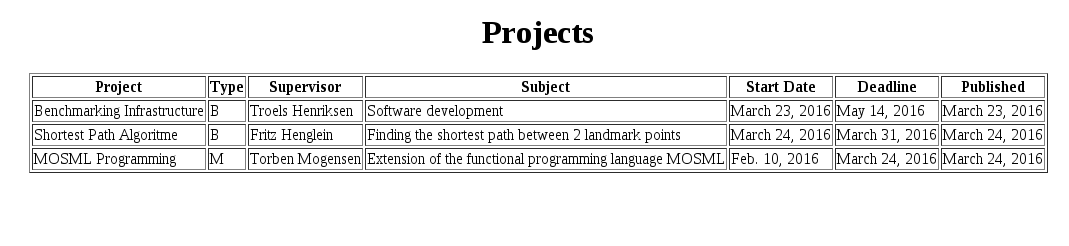
\includegraphics[width=1.0\textwidth]{projects.png}
			\caption{Forskellige projekter tilføjet til vores Django webapp.}
			\label{fig:projects}
\end{figure}
Ovenstående på figur\ref{fig:projects} kan man se nogle \textit{dummy} projekter, som vi manuelt har tilføjet til vores webapp. Dette har vi gjort for at kunne tilpasse templates, og visuelt kunne se hvordan vi vil repræsentere data inden vi begynder at scrape.
\subsection{Scraper}
Til denne test har vi kørt vores scraper på hjemmesiden over DIKU Ansatte: \url{http://www.diku.dk/Ansatte}, og høster information baseret på nogle foruddefinerede HTML-tags. Nedenstående er et udsnit af vores resultat. \\ \\
Scraperen gemmer endnu ikke noget information i nogen database, men sender den høstede information til stdout. Et eksempel på programmets output kan ses herunder:
\begin{lstlisting}
Name: Abelskov, Hjalte
Link: http://diku.dk/Ansatte?pure=da/persons/432412
None
Instruktor


None
Name: Abrahamsen, Mikkel
Link: http://diku.dk/Ansatte?pure=da/persons/289414
None
ph.d.-studerende


Name: E-mail
Link: http://diku.dk/Ansatte
None
Name: Adamaszek, Anna Maria
Link: http://diku.dk/Ansatte?pure=da/persons/506000
None
Postdoc
\end{lstlisting}
\subsection{Controller}
Testene er placeret i vores test-mappe, herinde har vi lavet 7 forskellige tests, som har til formål at vise om testene bliver klaret, hvad deres output er, og hvor hurtig testene er. Testene er beskrevet nedenfor:
\begin{itemize}
\item \textit{files\_test()}
  \begin{itemize}
  \item Beskrivelse: Laver en mappe og 3 filer, derefter bliver indholdet af filerne printet.
  \item Forventet output: Strengene som er blevet skrevet til filerne. En lang streng, og to små.
  \end{itemize}
\item \textit{folder\_test()}
  \begin{itemize}
  \item Beskrivelse: Laver en mappe kaldet \textit{test}, og placerer 3 mapper inde i denne mappe. Printer derefter alle undermapper i mappen \textit{test}.
  \item Forventet output: 3 mapper.
  \end{itemize}
\item \textit{last\_modified\_test()}
  \begin{itemize}
  \item Beskrivelse: Laver 3 filer, hvoraf den ene først bliver lavet med en forsinkelse på 1 sekund, og derefter bliver deres last modified timestamp printet.
  \item Forventet output: Deres tid siden epoch, og et convertet læseligt timestamp. Den ene skal være anderledes grundet delay.
  \end{itemize}
\item \textit{last\_modified\_comparison\_test()}
  \begin{itemize}
  \item Beskrivelse: Samme som overstående, men deres timestamps bliver sammenlignet.
  \item Forventet output: Mappe 1 og 2 giver True, mens mappe 1 og 3 giver False.
  \end{itemize}
\item \textit{files\_ext\_test()}
  \begin{itemize}
  \item Beskrivelse: Laver 4 filer, hvoraf den ene har en anden filtype. Derefter bliver alle filerne med den ene type printet, og derefter filer med den anden type.
  \item Forventet output: Først skriver den alle \textit{.txt}-filer og derefter den ene \textit{.dat}-fil.
  \end{itemize}
\item \textit{clear\_file\_test()}
  \begin{itemize}
  \item Beskrivelse: Laver en fil, skriver en streng til den, printer indeholdet og derefter sletter den alt i filen og printer dens nye indhold.
  \item Forventet output: Først har filen et indhold der bliver printet, og derefter intet indhold.
  \end{itemize}
\item \textit{socket\_test()}
  \begin{itemize}
  \item Beskrivelse: Opretter en socket, og prøver at hente indholdet af en webside, som vi har liggende på vores webserver (så den aldrig ændrer sig). Skriver indeholdet til en fil, som derefter bliver printet.
  \item Forventet output: Filen der bliver skrevet til, vil være identisk med den der ligger på webserveren.
  \end{itemize}
\end{itemize}
Testene bliver kørt lige efter hinanden. Før en test bliver kørt begynder vi at tage tid, som bliver printet når testen er færdig. Efter hver test er der en pause på 1 sekund for at gøre det lettere at læse outputtet, inden den næste test bliver kørt.
\subsubsection{Output}
Vores tests returnerer True eller False, så vi ved om testen er fejlet eller ej. \\ \\
Herunder vises et udsnit af test resultaterne:
\begin{lstlisting}
Starting files test!
Files test returned: True
Files test took: --- 0.000173807144165 seconds ---

Starting folder test!
Folder test returned: True
Folder test took: --- 0.000287055969238 seconds ---

Starting last modified test!
Last modified test returned: True
Last modified test took: --- 1.00135111809 seconds ---
\end{lstlisting}
Bemærk at Last modified test tager over et sekund, da den venter et sekund før den laver den tredje fil.
\section{Design}
Django benytter \textit{models} og hver model knytter sig til en enkelt tabel i den tilhørende database. En model i Django er en Python klasse. \\ I vores projekt benytter vi indtil videre klasserne \texttt{Supervisor} og \texttt{Project}. På Figur \ref{fig:modelUML} ses et UML diagram for klasserne \texttt{Supervisor} og \texttt{Project}.

\begin{figure}[H]
			\centering
			\includegraphics[width=1.0\textwidth]{modelUML.png}
			\caption{Foreløbelig UML diagram over vores klasser.}
			\label{fig:modelUML}
\end{figure}
~\\
Dette er på nuværende tidspunkt, hvordan vi forestiller os det kommer til at se ud. Der vil formentlig ske ændringer i fremtiden, når vi bliver mere bekendte med hvilke attributer, vi skal gemme.

\section{Planlægning af næste iteration}
Vi vil fokusere på tre \textit{use cases} i næste iteration. Disse \textit{use cases} er:
\begin{enumerate}
\subsection*{Forventes implementeret i næste iteration}
	\item \label{enum:katalog} Det skal være muligt at se et katalog over projekter.

	\item \label{enum:verifikation} Personer, der optræder på siden, skal kunne verificeres, hvis de eksempelvis ønsker at tilføje projekter eller foretage rettelser.

\subsection*{Påbegyndes i næste iteration}

	\item \label{enum:vejlederInfo} Systemet skal kunne præsentere aktuelle oplysninger om potentielle vejledere, herunder:
	\begin{itemize}
		\item Tidligere projekter.
		\item Forskningspublikationer.
		\item Kontaktoplysninger.
	\end{itemize}
\end{enumerate}

\subsection{Underopgaver for de udvalgte \textit{use cases}}
\subsubsection*{\textit{Use case} \ref{enum:katalog}}
\begin{itemize}
	\item Django \textit{modellen} for et projekt skal færdiggøres.
	\item Der skal laves en \textit{template} knyttet til denne model.
\end{itemize}

\subsubsection*{\textit{Use case} \ref{enum:verifikation}}
De specifikke detaljer, for verificeringen, skal overvejes og konkretiseres nærmere. Verificeringen skal foregå med mindst mulig adminstrativ vedligholdelse, men samtidig korrekt. Hvis den deles op i underopgaver er disse:
\begin{itemize}
	\item Der skal en password generering.
	\item Muligheden for oprettelse af en bruger, med prædefinerede valg, ud fra det høstede data.
\end{itemize}

\subsubsection*{\textit{Use case} \ref{enum:vejlederInfo}}
Den høstede information om vejlederne skal benyttes til automatisk at oprette et katalog over vejledere. Hver af disse vejledere skal herefter kunne overtages af de respektive vejledere med oprettelse af en Django-bruger.
\begin{itemize}
	\item Scraperen skal kunne omforme den høstede data til det korrekte format.
	\item En Django-bruger skal kunne knyttes til en vejleder i kataloget.
	\item En katalog-vejleder skal kunne "låses", således at indtastet information har højere prioritet end høstet information.
\end{itemize}
\end{document}
